\documentclass[aspectratio=1610]{beamer}
\usecolortheme{beaver}
\usepackage{graphicx}
\usepackage{minted}
\usepackage{varwidth}
\usepackage{tikz}
\usepackage{tikzscale}
\usepackage{color}
\usepackage{url}
\definecolor{carnelian}{rgb}{0.7, 0.11, 0.11}
\usetikzlibrary{trees,shapes,positioning,arrows,fit}
\usepackage{fontspec}
\newfontface{\unicodefont}{Linux Biolinum}
\newfontface{\altunicodefont}{Noto Sans}
\usepackage{hyperref}
\begin{document}
\title{An Introduction to ZFS}
\subtitle{A Solid Foundation for Your Data}
\author{Christian Schwarz}
\date{GPN16, 28.05.2016}
\titlegraphic{
\includegraphics[width=80pt]{assets/openzfs_logo.pdf}}
\maketitle
%
%\begin{frame}
%	\tableofcontents
%\end{frame}

\section{Introduction}
\begin{frame}{Introduction}
	Storing data on disk
	\pause
	\begin{itemize}
		\item spinning rust \pause (faulty) \pause
		\item phantom writes \pause
		\item bit rot \pause (\unicodefont{�}) \pause 
		\item flaky power \pause (fsck-y) \pause
		\item firmware bugs (happen) \pause
		
		\item volume management \pause (ugly) \pause
		\item partitioning \pause (inflexible)
		\item ... \pause
	\end{itemize}
\end{frame}

%%%%%%%%%%%%%%%%%%%%%%%%%%%%%%%%%%%%%%%%%%%%%%%%%%%%%%%%%%%%%%%%%%%%%%%%%%%%%%%%

\begin{frame}[fragile]{Example: SoftRAID + LVM + mkfs.ext4}
\begin{minted}{sh}
# create softraid / soft-mirror
mdadm -C /dev/md0 --name md0 \
    --level=mirror -n2 /dev/sda1 /dev/sdb1
# init LVM physical volumes
pvcreate /dev/md0
# create LVM logical volume group
vgcreate vg0 /dev/md0
# create LVM logical volume
lvcreate -L 100G vg0 -n root
# create file system on logical volume
mkfs.ext4 /dev/mapper/vg0-root
\end{minted}

\end{frame}

%%%%%%%%%%%%%%%%%%%%%%%%%%%%%%%%%%%%%%%%%%%%%%%%%%%%%%%%%%%%%%%%%%%%%%%%%%%%%%%%

\begin{frame}{Example: Softraid + LVM + mkfs.ext4}
	\begin{columns}
		\begin{column}{0.25\linewidth}
			
		\end{column}
		\begin{column}{0.5\linewidth}
			\begin{figure}
				\includegraphics[]{assets/layers/traditional}
				%\caption{Traditional File System Stack. Source: \cite{zfs2003} }
			\end{figure}			
		\end{column}
		\begin{column}{0.25\linewidth}
			
		\end{column}
	\end{columns}

\end{frame}

%%%%%%%%%%%%%%%%%%%%%%%%%%%%%%%%%%%%%%%%%%%%%%%%%%%%%%%%%%%%%%%%%%%%%%%%%%%%%%%%

\begin{frame}{Example: Softraid + LVM + mkfs.ext4}
	\begin{center}
	\Huge
	We can do better.
	\end{center}
\end{frame}

\begin{frame}{Example: ZFS}
	\begin{center}
		\Huge ZFS
	\end{center}
\end{frame}

%%%%%%%%%%%%%%%%%%%%%%%%%%%%%%%%%%%%%%%%%%%%%%%%%%%%%%%%%%%%%%%%%%%%%%%%%%%%%%%%

\begin{frame}[fragile]{Example: ZFS} 
\begin{minted}{sh}
# create storage pool
# implicitly creating root filesystem
zpool create tank mirror /dev/sda1 /dev/sdb1
\end{minted}
\end{frame}

%%%%%%%%%%%%%%%%%%%%%%%%%%%%%%%%%%%%%%%%%%%%%%%%%%%%%%%%%%%%%%%%%%%%%%%%%%%%%%%%

\begin{frame}[fragile]{Example: ZFS} 
\begin{minted}{sh}
zpool status tank

  pool: tank
  state: ONLINE
  scan: none requested
  config:
  
  NAME            STATE     READ WRITE CKSUM
  tank            ONLINE       0     0     0
    mirror-0      ONLINE       0     0     0
      /dev/sda1   ONLINE       0     0     0
      /dev/sdb1   ONLINE       0     0     0
\end{minted}
\end{frame}


\section{Design}
\begin{frame}{}
\begin{center}
	\Huge ZFS
\end{center} 
\end{frame}

\begin{frame}{ZFS Design Goals}
	\begin{itemize}
		\item Simple Administration
		\item Pooled Storage
		\item Always Consistent On-Disk State
		\item Error Detection And Correction
	\end{itemize}	
\end{frame}

\begin{frame}[allowframebreaks]{ZFS Features}
	%\note{Many ZFS Features are a byproduct of the implementation chosen to achieve the aforementioned design goals}
	\begin{itemize}[]
		\item No \texttt{fsck}. Ever.
		\item Simple Interface
		\begin{itemize}
			\item Inheritance Model
			\item Delegate Datasets to Unprivileged Users
			\item Delegate Datasets to Zones / Jails
		\end{itemize}
		\item Disk-level redundancy
		\item Data-integrity
		\item Dynamically allocated POSIX file systems
		\item Quotas \& Reservations %\note{Storage management}
		\framebreak
		\item ZVOLs - ZFS-backed block devices %\note{iSSCI}
		\item Cheap, Consistent Copy-on-Write Snapshots \& Clones
		\item Fast Replication \& Backups
		\item Per-Dataset configurable Compression \& Deduplication
		\item Hybrid Storage Model
		\item Variable Block-Size
		\framebreak
		\item ...
	\end{itemize}
\end{frame}



\section{Implementation}
\begin{frame}
	\begin{center}
		\Huge Implementation
	\end{center}
\end{frame}

\subsection{Layers in Comparison}
\subsubsection{Traditional}
\begin{frame}[label=overview_traditional_layering]{Overview: Traditional Layering}
	\begin{columns}[c]
		\begin{column}{0.4\textwidth}
			\begin{figure}
				\centering
				\includegraphics[height=0.6\textheight]{assets/layers/traditional}
			%	\caption{ \small Traditional: \cite{zfs2003} }
			\end{figure}
		\end{column}
		\pause
		\begin{column}{0.4\textwidth}
			\begin{itemize}
				\item<5-> System Call: interface to applications
				\item<4-> File System: on-disk data format %only in this sense, a file system is much more, of course, e.g. an organizational abstraction
				\item<3-> Volume Manager: volume abstraction
				\item<2-> Device Driver: hardware abstraction
			\end{itemize}
		\end{column}
	\end{columns}
\end{frame}

\begin{frame}{Traditional: Example On-Disk Format}
	\begin{figure}
	\centering
	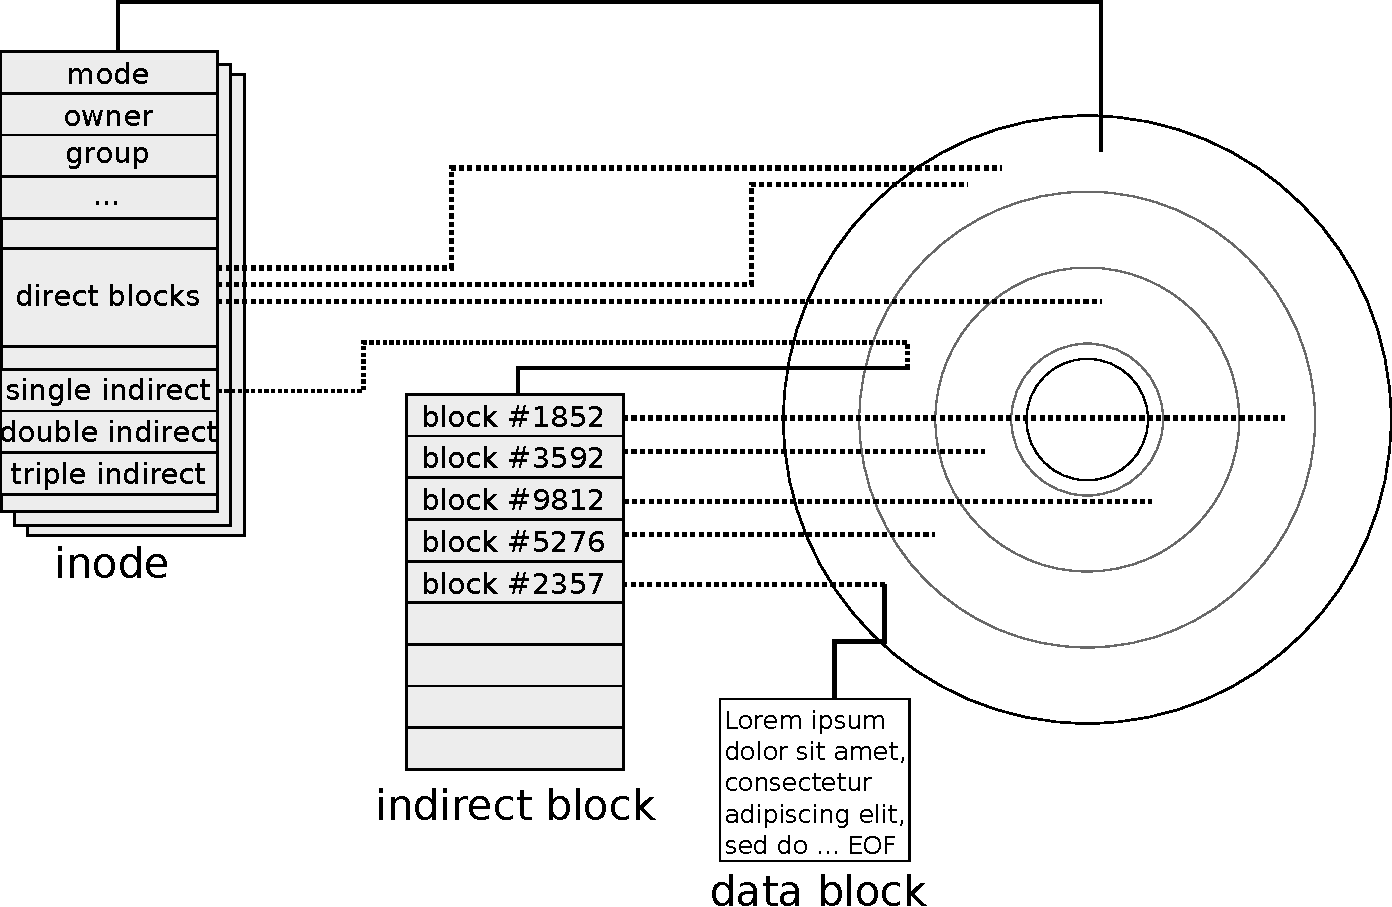
\includegraphics[height=0.75\textheight]{assets/traditional_fs}
	\end{figure}
\end{frame}

\begin{frame}{Traditional: Example \texttt{read}(3) \& \texttt{write}(3)}
	\begin{figure}
		\centering
		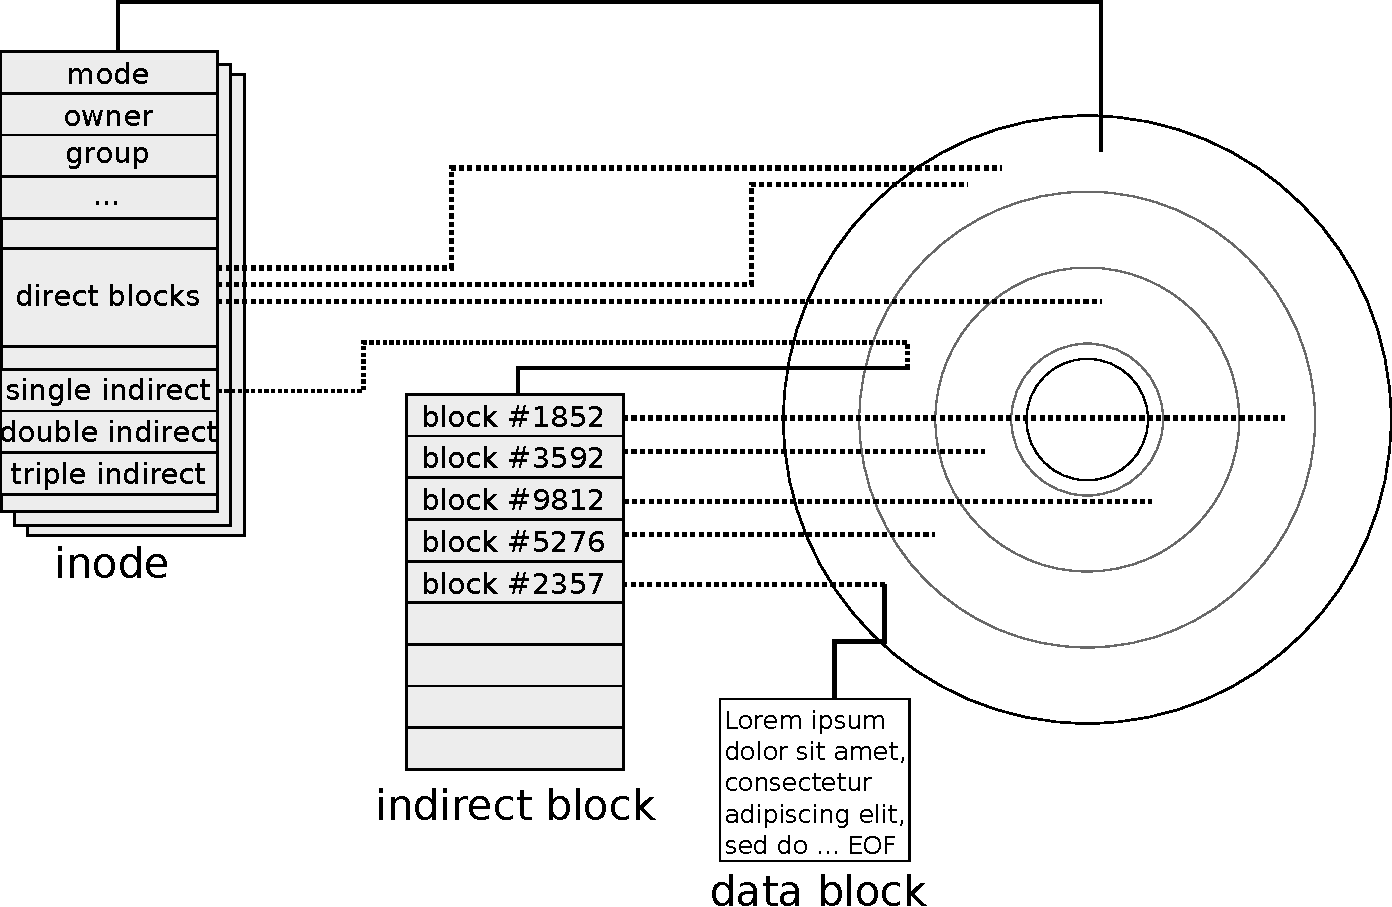
\includegraphics[height=0.75\textheight]{assets/traditional_fs}
	\end{figure}
\end{frame}

\againframe<6->{overview_traditional_layering}
\begin{frame}{Comparison: Traditional vs. ZFS}
		\begin{columns}[c]
			\begin{column}{0.4\textwidth}
				\begin{figure}
					\centering
					\includegraphics[height=0.7\textheight]{assets/layers/traditional}
				%	\caption{ \small Traditional: \cite{zfs2003} }
				\end{figure}
			\end{column}
			\begin{column}{0.4\textwidth}
				\begin{figure}
					\centering
					\includegraphics[height=0.7\textheight]{assets/layers/zfs}
				%	\caption{ \small ZFS: \cite{zfs2003} }
				\end{figure}
			\end{column}
		\end{columns}
\end{frame}

\subsubsection{ZFS}
\begin{frame}[label=overview_zfs_stack]{ZFS Layers}
	\begin{columns}[c]
		\begin{column}{0.4\textwidth}
			\pause
			\begin{itemize}
				\onslide+<4->
				\item ZFS Posix Layer
				\begin{itemize}
					\item File Systems
				\end{itemize}
				\onslide+<3->	
				\item Data Management Unit
					\begin{itemize}
						\item Transactions
						\item Flat Objects
					\end{itemize}
				\onslide+<2->
				\item Storage Pool Allocator
				\begin{itemize}
					\item \small DVA Abstraction % Later
					\item \small Disk Redundancy
					\item \small IO Orchestration
				\end{itemize}
			\end{itemize}
		\end{column}
			\onslide+<0->
			\begin{column}{0.4\textwidth}
				\begin{figure}
					\centering
					\includegraphics[height=0.7\textheight]{assets/layers/zfs_differences}
				\end{figure}
			\end{column}
	\end{columns}
\end{frame}

% Start explaining ZFS implementation by walking up the low-level ZFS layers
\subsection{Basic Concepts}
\begin{frame}{ZFS Basic Concepts}
	\begin{center}
		\Huge ZFS Basic Concepts
	\end{center}	
\end{frame}


\begin{frame}<6->[label=impl_tech_overview]
	\frametitle{ZFS Basic Concepts}
	{\Large Key Techniques}\\
	\begin{itemize}
		\item \alert<2>{Block-Pointers}
		\item \alert<3>{Tree-Structure}
		\item \alert<4>{Block-Level Checksumming}
		\item \alert<5>{Copy-on-Write}
	\end{itemize}
\end{frame}

\againframe<2>{impl_tech_overview}
\subsubsection{Block-Pointers}
\begin{frame}{Block-Pointers}
	\begin{figure}
	\centering
	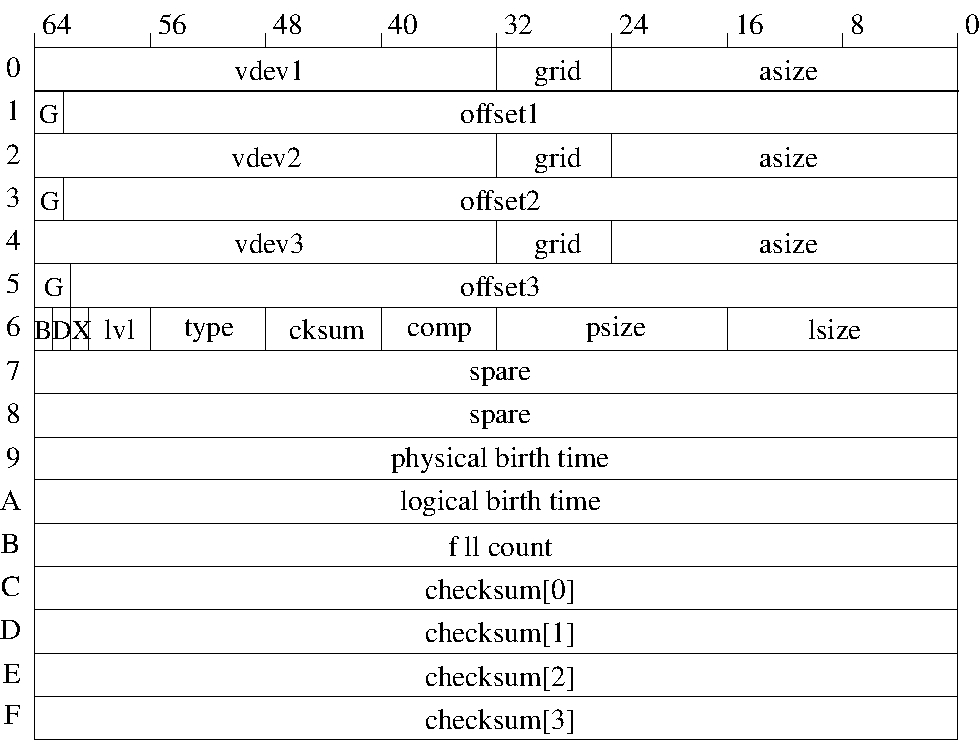
\includegraphics[height=0.75\textheight]{assets/on_disk/block_pointer}
	\caption{ZFS Block Pointer. Source \cite{introimplzfs}}
	\end{figure}
\end{frame}

\againframe<3>{impl_tech_overview}
\subsubsection{Tree Structure}
\begin{frame}{Tree Structure}
	\begin{figure}
	\centering
	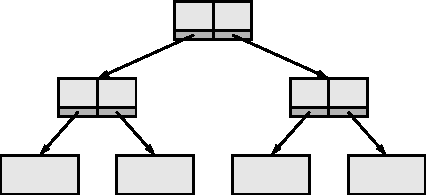
\includegraphics[width=0.6\linewidth]{assets/on_disk/tree_structure}
	\caption{Tree Structure. Source \cite{zfs2003}}
	\end{figure}
\end{frame}

\againframe<4>{impl_tech_overview}
\subsubsection{Block-Level Checksumming}
\begin{frame}{Block-Level Checksumming}
	\begin{figure}
		\centering
		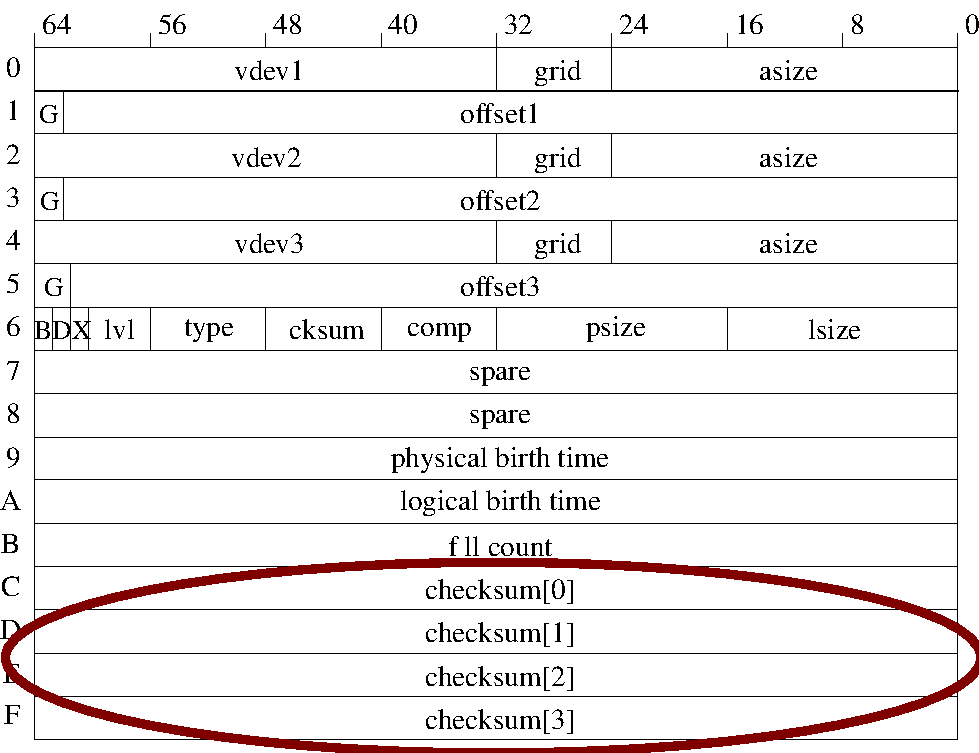
\includegraphics[height=0.75\textheight]{assets/on_disk/block_pointer_checksum_highlighted}
		\caption{ZFS Block Pointer. Source \cite{introimplzfs}}
	\end{figure}
\end{frame}

\againframe<5>{impl_tech_overview}
\subsubsection{Copy-on-Write}
\begin{frame}{Copy-on-Write}
\begin{columns}
	\begin{column}{0.4\textwidth}
			\begin{itemize}
				\item<2-> Modify Data Block \\ $\implies$ Write Copy
				\item<3-> Checksum Changes
				\item<4-> Modify $1^{st}$ level indirect block \\ $\implies$ Write Copy
				\item<5-> Ripple, ripple, ripple...
				\item<6-> Overwrite \alert{Überblock} in-place$^*$
			\end{itemize}
	\end{column}
	\begin{column}{0.6\textwidth}
		\begin{figure}
		\centering
		\only<1>{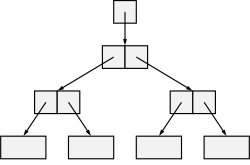
\includegraphics[width=\linewidth]{assets/on_disk/cow/begin}}
		\only<2-3>{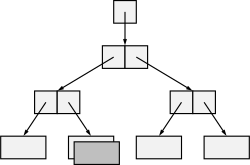
\includegraphics[width=\linewidth]{assets/on_disk/cow/data_block}}
		\only<4>{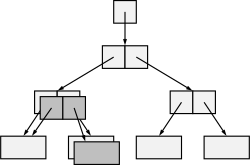
\includegraphics[width=\linewidth]{assets/on_disk/cow/first_indirect}}
		\only<5>{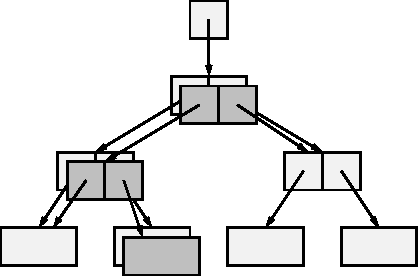
\includegraphics[width=\linewidth]{assets/on_disk/cow/second_indirect}}
		\only<6>{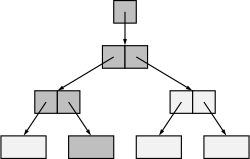
\includegraphics[width=\linewidth]{assets/on_disk/cow/uberblock}}
		\caption{ZFS Copy-on-Write. Source \cite{zfs2003}}
	\end{figure}
	\end{column}
\end{columns}
\end{frame}

%%%%%%%%%%%%%%%%%%%%%%%%%%%%%%%%%%%%%%%%%%%%%%%%%%%%%%%%%%%%%%%%%%%%%%%%%%%%%%%%

% This is a crippling analogy to legacy filesystems
% Let's look at a more complete picture
\subsection{ZFS Modules}
\begin{frame}{ZFS Modules}
	\begin{center}
		\Huge ZFS Modules
	\end{center}	
\end{frame}

\begin{frame}[label=zfs_module_layering]{ZFS Modules}
	\begin{figure}
		\centering
		\includegraphics[height=0.85\textheight]{assets/zfs_modules}
	%	\caption{ \small ZFS module layering. Source \cite{difbsd2nd} }
	\end{figure}
\end{frame}

% We walk bottom up, exploring the functionality each module provides

\subsubsection{VDEVs}
\begin{frame}[fragile]{VDEVs}
	\begin{columns}
		\begin{column}{0.5\linewidth}
				\begin{itemize}
					\item SPA \emph{stripes} root VDEVs
					\item VDEVs implement
					\begin{itemize}
						\item Access to Physical Storage
						\item Disk Redundancy
					\end{itemize}
					\item Building-block approach
					\item Nesting
				\end{itemize}
		\end{column}
		\begin{column}{0.5\linewidth}
			\visible<2->{
				\begin{figure}
				\centering
				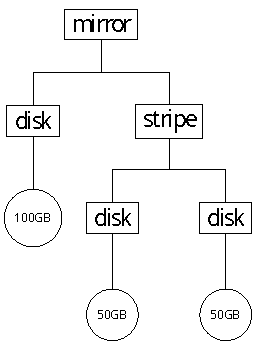
\includegraphics[height=0.3\textheight]{assets/zpool_vdev_nesting_own}
				\caption{Nested VDEVs.}
				\end{figure}
			}
		\end{column}
	\end{columns}
	\vspace{20pt}
% Need to keep this to the left or alternatively use spaces
\begin{columns}<3->
\begin{column}{0.4\textwidth}
\centering
\begin{varwidth}{0.4\linewidth}
\begin{semiverbatim}
vdev_\alert{disk}.c
vdev_\alert{geom}.c
vdev_\alert{file}.c
vdev_\alert{cache}.c
vdev_label.c
\end{semiverbatim}
\end{varwidth}
\end{column}
\begin{column}{0.4\textwidth}
\centering
\begin{varwidth}{0.4\linewidth}
\begin{semiverbatim}
vdev_\alert{mirror}.c
vdev_\alert{raidz}.c
vdev_missing.c
vdev_queue.c
vdev_root.c
\end{semiverbatim}
\end{varwidth}
\end{column}
\end{columns}
\end{frame}

\begin{frame}{VDEVs: Disk Redundancy}
\begin{itemize}
	\item Mirroring
	\item RAIDZ-1 $\approx$ RAID-(3|5)ish with logical blocks
	\item RAIDZ-2, RAIDZ-3
	\item Checksumming \\
	$\implies$ Protect Against RAID-5 \emph{Write-Hole}
	\item Fast \emph{resilvering} on moderately filled pools % because can walk tree and only copy indirect blocks (like logical backups, not a dump)
\end{itemize}
\end{frame}

\subsubsection{Storage Pool Allocator (SPA)}
\begin{frame}{Storage Pool Allocator (SPA)}
	Implements \vspace{10pt}
	\begin{itemize}
		\item Checksumming
		\item Compression
		\item Block-level Deduplication
		\item Disk Redundancy (VDEVs)
		\item ZIO: IO Orchestration \& Prioritization %fsyncs need to get to intent-log quickly, while asynchronous txg_groups are lower prio.
	\end{itemize}
	\vspace{10pt}
	Exposes DVA interface $\approx$ \texttt{malloc}(3) \texttt{free}(3)
\end{frame}

\againframe{zfs_module_layering}
\subsubsection{Data Management Unit (DMU)}
\begin{frame}[fragile,allowframebreaks]{Data Management Unit (DMU)}
	\begin{itemize}
	\item Objects with file-like interface \\ \texttt{(objectid, offset)}
	\item Private Namespace (object set / \emph{dataset}) \\ \texttt{(\alert{object set}, objectid, offset)}
	\item Create / Read / Write / Delete objects in Transactions
	\end{itemize}
\pagebreak
\small
\vspace{-2em}
\begin{minted}{c}
/*
 * You must create a transaction, then hold the objects
 * which you will (or might) modify as part of this
 * transaction. Then you must assign the transaction 
 * to a transaction group. Once the transaction has
 * been assigned, you can modify buffers which belong to
 * held objects as part of this transaction. [...]
 */
dmu_tx_t *dmu_tx_create(objset_t *os);
void dmu_tx_commit(dmu_tx_t *tx);
void dmu_tx_abort(dmu_tx_t *tx);

void dmu_write(objset_t *os, uint64_t object, uint64_t offset,
               uint64_t size, const void *buf, dmu_tx_t *tx);
               
void dmu_prealloc(objset_t *os, uint64_t object,
                  uint64_t offset, uint64_t size, dmu_tx_t *tx);
\end{minted}
\centering
\tiny \hfill Lines from \cite{openzfssrc_dmu}
\end{frame}

\againframe{zfs_module_layering}
\subsubsection{Dataset- \& Snapshot Layer (DSL)}
\begin{frame}[allowframebreaks]{Dataset- \& Snapshot Layer (DSL) + Meta-Object Set}
	DMU used for different purposes \vspace{10pt}
	\begin{itemize}
		\item POSIX filesystems (ZPL) % with POSIX semantics
		\item ZVOLs (DMU-backed block device)
		\item Snapshots (consistent state of FS / ZVOL)
		\item Clones (rw filesystem starting off snapshot)
		\item \texttt{\$APP} (maybe, someday)
	\end{itemize}  \vspace{10pt}
	$\implies$ Need container for object sets $\implies$ \alert{meta-object set}
	\pagebreak
	\begin{figure}
	\centering
	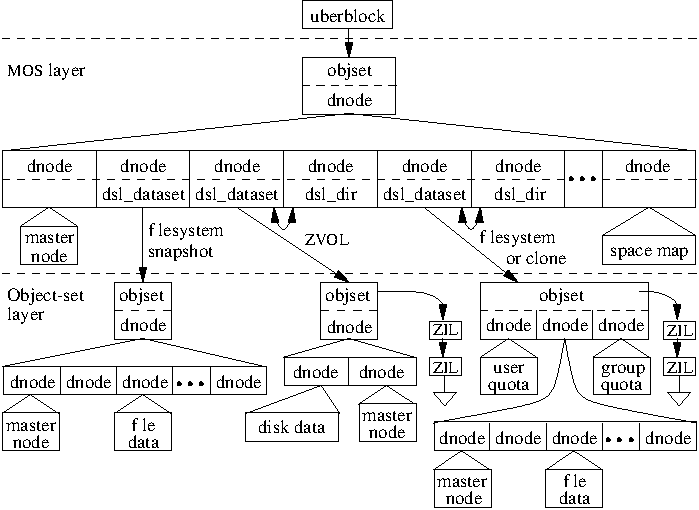
\includegraphics[height=0.75\textheight]{assets/on_disk/detailed_with_dsl_structures}
	\caption{On-Disk Structures, including MOS. Source \cite{introimplzfs}}
	\end{figure}
\end{frame}

\againframe{zfs_module_layering}
\subsubsection{Adaptive Replacement Cache (ARC) \& L2ARC}
\begin{frame}{Adaptive Replacement Cache (ARC) \& L2ARC}
\begin{itemize}
	% This is why ZFS is performant (at all)
	\item Adaptive Replacement Cache
	\begin{itemize}
		\item Physically Indexed (SPA-)Block-level Cache % Physical = ZFS-Block-Level, i.e. the blocks pointed to by block pointers => Physical saves resources because block is shared between live filesystem and its snapshots & clones, etc.
		\item Scan-resistant LRU eviction strategy % Based on an algorithm from IBM research. Uses combination of MRU and MFU + tracking of eviction + adjustment of MRU/MFU size in response to eviction tracking
		\item Separate from system page cache % result of ZFS's monolithic design. Easier portability, but things like mmap & sendfile waste memory
		\item Will eat up all$^*$ your memory
	\end{itemize}
	\item L2ARC = Level 2 ARC % expand the ARC to secondary storage, e.g. a fast SSD in a HDD-only pool
\end{itemize}
\end{frame}

\againframe{zfs_module_layering}
\subsubsection{ZFS POSIX Layer (ZPL)}
\begin{frame}{ZFS POSIX Layer (ZPL)}
	\begin{itemize}
		\item File Systems with POSIX Semantics
		\pause
		\begin{itemize}
			\item Directories
			\item Files
			\item Permissions
			\item ACLs
			\item xattr
			\item ...
		\end{itemize}
		\pause
		\item $\implies$ Leverage DMU + ZAP + ZIL
	\end{itemize}
\end{frame}

\againframe{zfs_module_layering}
\subsubsection{ZFS Attribute Processor (ZAP)}
\begin{frame}{ZFS Attribute Processor (ZAP)}
	\begin{itemize}
		\item $\approx$ Key-Value Data Store / dictionary$^*$ % Can have nested structures
		\item Store metadata
		\begin{itemize}
			\item File Attributes (ZPL)
			\item Directories (ZPL)
			\item Dataset Attributes (DSL)
			\item Pool Attributes
			\item ...
		\end{itemize}
	\end{itemize}
\end{frame}

\subsubsection{ZFS Intent Log (ZIL)}
\begin{frame}{ZFS Intent Log (ZIL)}
\begin{itemize}
	\item $\approx$ Journaling for ZPL \& ZVOLs
	\item POSIX Atomic Transactions without DMU checkpoint %remember: DMU cares about on-disk consistency. Does this with checkpoints (transaction groups) that group transactions. Checkpoints are not written frequently enough to use them for fsync(3).
	\item Can designate specific VDEV %mitigate write performance bootleneck / increase write IOPs
\end{itemize}
\end{frame}

\againframe{zfs_module_layering}
\subsubsection{ZFS Volume (ZVOL)}
\begin{frame}{ZFS Volume (ZVOL)}
	\begin{itemize}
		\item DMU backed block storage
		\item Export via iSCSI
		\item Local \& Remote VM Storage %With all the goodness of the lower layers
	\end{itemize}
\end{frame}

\againframe{zfs_module_layering}
\subsubsection{/dev/zfs}
\begin{frame}{/dev/zfs}
	\begin{itemize}
		\item \texttt{zpool}(8) \& \texttt{zfs}(8)
		\item \texttt{ioctl}(2) to \texttt{/dev/zfs}
		\item Configure VDEVs
		\item Send \& Receive Snapshot Streams % As introduced earlier: very fast & convenient dataset replication
	\end{itemize}
\end{frame}

\againframe{zfs_module_layering}

%%%%%%%%%%%%%%%%%%%%%%%%%%%%%%%%%%%%%%%%%%%%%%%%%%%%%%%%%%%%%%%%%%%%%%%%%%%%%%%%

\subsection{Example}
\begin{frame}{ZFS Modules - Example}
	\begin{center}
		\Huge Example
	\end{center}	
\end{frame}

\begin{frame}{\texttt{write}(3)}
\begin{figure}
	\centering
	\includegraphics[height=0.7\textheight]{assets/zfs_modules}
\end{figure}
\end{frame}

%%%%%%%%%%%%%%%%%%%%%%%%%%%%%%%%%%%%%%%%%%%%%%%%%%%%%%%%%%%%%%%%%%%%%%%%


\section{ZFS in Action}
\begin{frame}{ZFS in Action}
	\begin{center}
		\Huge ZFS in Action
	\end{center}
\end{frame}
%
\begin{frame}{ZFS in Action}
	\begin{itemize}
		\item Create Disks 0 5
		\item Create mirrored stripes
		\item zpool status
		\item Create spare zpool add spare
		\item Create text file
		\item Watch zpool 
		\item Corrupt one disk's data (dd if=/dev/random of=/tmp/diski bs=1k seek=256 count=100k)
		\item Scrub
		\item Watch Zpool report checksumming corrections
		\item watch zpool status tank
		\item Shred a disk (where uberblocks are kept) (dd if=/dev/urandom of=/tmp/diski bs=1M count=100 )
		\item scrub
		\item Do zpool replace (watch zpool status)
		\item watch zpool status change
		\item watch zfs list
		\item zfs create
		\item zfs create -o compression=on
		\item create compressible file, dd if=/dev/zero of=/mountpoint/zeroes bs=1M count=300M
		\item zfs snapshot ds@snap1
		\item zfs list -t snapshot ds
		\item delete /mountpoint/zeroes
		\item zfs diff ds@snap1 ds
		\item talk about backup solutions
		\item zpool create backups mirror /tmp/disk4 /tmp/disk5
		\item zfs snapshot -v -r ds@initial\_backup
		\item zfs send -R ds@initial\_backup | zfs receive backups
		\item zfs list -t snapshot backups
		\item mention that pipe could traverse networks, e.g. with SSH
	\end{itemize}
\end{frame}

\section{Availibility}
\begin{frame}{Supported Platforms}
		\begin{columns}
			\begin{column}{0.5\linewidth}
				\begin{itemize}
					\item OpenZFS on OS X
					\item FreeBSD and derivatives
					\item Illumos
					\item Linux
				\end{itemize}
				\vspace{2em}
				$\implies$ \url{http://open-zfs.org}
			\end{column}
			\begin{column}{0.5\linewidth}
				\begin{figure}
					\centering
					
\includegraphics[height=0.4\textheight]{assets/contrib/openzfs/openzfs_logo}
				\end{figure}
			\end{column}
		\end{columns}
\end{frame}

\section{Workshop}
\begin{frame}{Workshop}
	\centering
	\huge
	Workshop \textit{ZFS for Beginners} \\
	Sat, 28.05.2016, \alert{18:00} \\
	Kleiner Workshopraum
\end{frame}

\section{Credits \& References}
\begin{frame}[allowframebreaks]{Credits \& References}
	\nocite{*}
	\bibliographystyle{ieeetr}
	\bibliography{bibliography}
\end{frame}

\section{Reusing Materials}
\begin{frame}[allowframebreaks]{Reusing Materials from this Talk}
\centering
Please check \texttt{README.md} at \url{https://perma.cschwarz.com/talks/introzfs2016}.
\end{frame}

\end{document}
